\documentclass[UTF8]{ctexart}
\usepackage{geometry, CJKutf8}
\geometry{margin=1.5cm, vmargin={0pt,1cm}}
\setlength{\topmargin}{-1cm}
\setlength{\paperheight}{29.7cm}
\setlength{\textheight}{25.3cm}
\setlength{\headheight}{12.64723pt}


% useful packages.
\usepackage{amsfonts}
\usepackage{amsmath}
\usepackage{amssymb}
\usepackage{amsthm}
\usepackage{enumerate}
\usepackage{graphicx}
\usepackage{multicol}
\usepackage{fancyhdr}
\usepackage{layout}
\usepackage{listings}
\usepackage{float, caption}
\usepackage{xcolor}
\usepackage{tikz}
\usepackage{tikz-qtree}

\lstset{
    basicstyle=\ttfamily, basewidth=0.5em,
    language=C++,
    keywordstyle=\color{blue},
    stringstyle=\color{green},
    commentstyle=\color{gray},
    numbers=left,
    numberstyle=\ttfamily\color{gray}\footnotesize,
    stepnumber=1,
    breaklines=true,
    showstringspaces=false,
    tabsize=4
}

% some common command
\newcommand{\dif}{\mathrm{d}}
\newcommand{\avg}[1]{\left\langle #1 \right\rangle}
\newcommand{\difFrac}[2]{\frac{\dif #1}{\dif #2}}
\newcommand{\pdfFrac}[2]{\frac{\partial #1}{\partial #2}}
\newcommand{\OFL}{\mathrm{OFL}}
\newcommand{\UFL}{\mathrm{UFL}}
\newcommand{\fl}{\mathrm{fl}}
\newcommand{\op}{\odot}
\newcommand{\Eabs}{E_{\mathrm{abs}}}
\newcommand{\Erel}{E_{\mathrm{rel}}}

\begin{document}

\pagestyle{fancy}
\fancyhead{}
\lhead{吴慧阳  3230105143}
\chead{数据结构与算法第五次作业}
\rhead{\today}

\section{\texttt{remove}函数的实现思路}
我们使用一颗具体的二叉树来说明我们是如何实现\texttt{remove()}函数的.
\par
\begin{center}

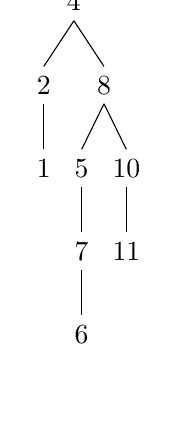
\begin{tikzpicture}
    \Tree
      [.4
        [.2
          [.1 ]
        ]
        [.8
          [.5
            [.7
              [.6 ]
            ]
          ]
          [.10
            [.11 ]
          ]
        ]
      ]
  \end{tikzpicture}     
\end{center}
按照提示,我们先构造了一个\texttt{detachMin()}函数用以
查找以 t 为根的子树中的最小节点,
返回这个节点,并从原子树中删除这个节点。显然,
当要删除的节点具有两个子树时,通过这个函数
返回的右子树最小节点将代替被删除节点。
具体而言,我们如果需要删除以\texttt{8}为根的子树中的最小节点,
\texttt{detachMin()}函数会返回\texttt{5},并将\texttt{7}
接到\texttt{8}的左节点处.\par
此时二叉树变成\par
\begin{center}

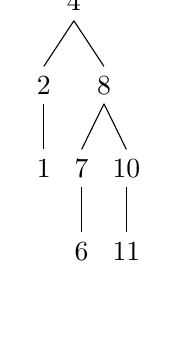
\begin{tikzpicture}
    \Tree
      [.4
        [.2
          [.1 ]
        ]
        [.8
          [.7
            [.6 ]
          ]
          [.10
            [.11 ]
          ]
        ]
      ]
  \end{tikzpicture}     
\end{center}
在理解了\texttt{detachMin()}的功能后,我们可以实现\texttt{remove()}
的功能了,具体实现如下:
\begin{lstlisting}
    BinaryNode *detachMin (BinaryNode *&t) 
    {
   if (t == nullptr) return nullptr;
   if (t->left == nullptr)
   { BinaryNode *minNode = t;
   t = t->right;
   return minNode;
   }
   return detachMin(t->left);
    }
    void remove (const Comparable &x, BinaryNode *&t) 
    {
    if (t == nullptr) return;
    if (x > t->element) remove(x, t->right);
    else if (x < t->element) remove(x, t->left);
    else
        {
        if (t->left == nullptr) 
            {
            BinaryNode *oldNode = t;
            t = t->right;
            delete oldNode;
            }
        else if (t->right == nullptr) 
            {
            BinaryNode *oldNode = t;
            t = t->left;
            delete oldNode;
            }
        else
            {
            BinaryNode *minNode = detachMin(t->right);
            minNode->left = t->left;
            minNode->right = t->right;
            delete t;
            t = minNode;
            }
        }
    }

\end{lstlisting}
例如,当我们对前文的二叉树运行\texttt{remove(4)}时,
\texttt{detachMin()}函数先将二叉树化为
\par
\begin{center}

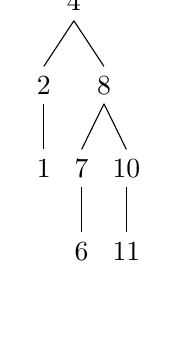
\begin{tikzpicture}
    \Tree
      [.4
        [.2
          [.1 ]
        ]
        [.8
          [.7
            [.6 ]
          ]
          [.10
            [.11 ]
          ]
        ]
      ]
  \end{tikzpicture}     
\end{center}
然后剩余的代码用\texttt{5}替代了根节点\texttt{4}.
从而二叉树最后变成\par
\begin{center}

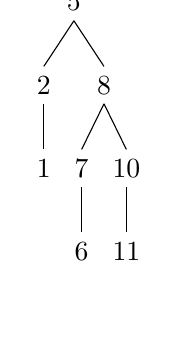
\begin{tikzpicture}
    \Tree
      [.5
        [.2
          [.1 ]
        ]
        [.8
          [.7
            [.6 ]
          ]
          [.10
            [.11 ]
          ]
        ]
      ]
  \end{tikzpicture}     
\end{center}
这仍然是一个BST.
如果我们最初选择删除叶子\texttt{1},则二叉树变为
\par
\begin{center}

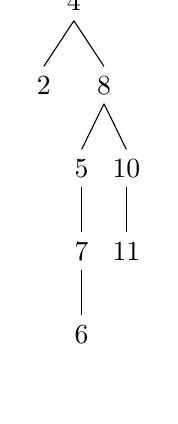
\begin{tikzpicture}
    \Tree
      [.4
        [.2 ]
        [.8
          [.5
            [.7
              [.6 ]
            ]
          ]
          [.10
            [.11 ]
          ]
        ]
      ]
  \end{tikzpicture}     
\end{center}
类似的,在最初分别选择删除\texttt{2}(只有左子节点的节点)、
\texttt{10}(只有右子节点的节点)\texttt{8}(有左右子节点的节点)
后得到的二叉树分别为\par
\begin{center}

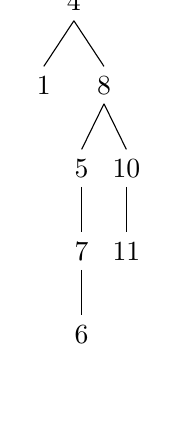
\begin{tikzpicture}
    \Tree
      [.4
        [.1 ]
        [.8
          [.5
            [.7
              [.6 ]
            ]
          ]
          [.10
            [.11 ]
          ]
        ]
      ]
  \end{tikzpicture}     
\end{center}
\par
\begin{center}

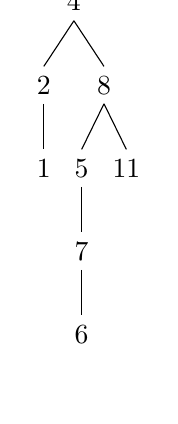
\begin{tikzpicture}
    \Tree
      [.4
        [.2
          [.1 ]
        ]
        [.8
          [.5
            [.7
              [.6 ]
            ]
          ]
          [.11 ]
        ]
      ]
  \end{tikzpicture}     
\end{center}
\par
\begin{center}

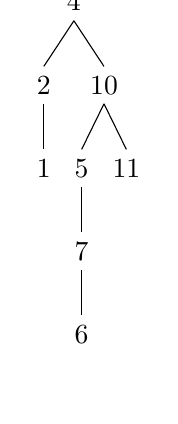
\begin{tikzpicture}
    \Tree
      [.4
        [.2
          [.1 ]
        ]
        [.10
          [.5
            [.7
              [.6 ]
            ]
          ]
          [.11
          ]
        ]
      ]
  \end{tikzpicture}     
\end{center}
\section{测试程序}
刚才的图示用代码表示如下
\begin{lstlisting}
    void testBinarySearchTree() {
    BinarySearchTree<int> bst;

    bst.insert(4);
    bst.insert(2);
    bst.insert(8);
    bst.insert(5);
    bst.insert(1);
    bst.insert(7);
    bst.insert(6);
    bst.insert(10);
    bst.insert(11);
    bst.printTree();
    BinarySearchTree<int> bst_1 = bst;
    BinarySearchTree<int> bst_2 = bst;
    BinarySearchTree<int> bst_3 = bst;
    BinarySearchTree<int> bst_4 = bst;
    BinarySearchTree<int> bst_5 = bst;
    BinarySearchTree<int> bst_6;

    std::cout << "Delete a node with no child : " << std::endl;
    bst_1.remove(1);
    bst_1.printTree();

    std::cout << "Delete a node with a left child : " << std::endl;
    bst_2.remove(2);
    bst_2.printTree();

    std::cout << "Delete a node with a right child : " << std::endl;
    bst_3.remove(10);
    bst_3.printTree();

    std::cout << "Delete a node with both right and left child : "<< std::endl;
    bst_4.remove(8);
    bst_4.printTree();
    std::cout << "Delete a node twice : "<< std::endl;
    bst_4.remove(8);
    bst_4.printTree();

    std::cout << "Delete a nonexisting node : "<< std::endl;
    bst.remove(111);
    bst.printTree();
    
    std::cout << "Delete a root node : "<< std::endl;
    bst_5.remove(4);
    bst_5.printTree();
    
    std::cout << "Delete a node of an empty tree : " << std::endl;
    std::cout << "Before deletion : " << std::endl;
    bst_6.printTree();
    std::cout << "After deletion : " << std::endl;
    bst_6.remove(1);
    bst_6.printTree();
}
\end{lstlisting}
可以看到,我们还额外测试了对空树\texttt{remove()}的结果.

\section{测试的结果}
编译后,结果如下:
\begin{lstlisting}
1
2
4
5
6
7
8
10
11
Delete a node with no child : 
2
4
5
6
7
8
10
11
Delete a node with a left child : 
1
4
5
6
7
8
10
11
Delete a node with a right child : 
1
2
4
5
6
7
8
11
Delete a node with both right and left child : 
1
2
4
5
6
7
10
11
Delete a node twice : 
1
2
4
5
6
7
10
11
Delete a nonexisting node : 
1
2
4
5
6
7
8
10
11
Delete a root node : 
1
2
5
6
7
8
10
11
Delete a node of an empty tree : 
Before deletion : 
Empty tree
After deletion : 
Empty tree

\end{lstlisting}
符合预期结果.
\end{document}

%%% Local Variables: 
%%% mode: latex
%%% TeX-master: t
%%% End: 
